\documentclass[10pt]{beamer}
% \usetheme{}
\usecolortheme{beaver}

\usepackage[greek, english]{babel}
\usepackage{fontspec}
\setsansfont{DejaVuSansMono Nerd Font}

\setbeamersize{text margin left=10mm,text margin right=10mm}

\usepackage{graphicx}
\usepackage{changepage}

\title{Εφαρμογή Διαχείρησης Σταθμών Φόρτισης Ηλεκτρικών Αυτοκινήτων}
\author{Αλυσσανδράκης Νικόλαος-Αλκίνοος(1072752)\newline ~Φιλιππάτος Νικόλας(1072754)}
\date{10-1-2023}

\begin{document}

\begin{frame}
    \titlepage
\end{frame}

\begin{frame}
    \frametitle{Μικρόκοσμος(1/2)}

    Μας ζητήθηκε να φτιάξουμε μια εφαρμογή που διαχειρίζεται σταθμούς φόρτισης ηλεκτρικών αυτοκινήτων.\newline

    Οι σταθμοί φόρτισης βρίσκονται σε διάφορες περιοχές με open location codes για εύκολη αναζήτηση και έχουν συγκεκριμένο αριθμό φορτιστών (θέσεων).\newline

    Κάθε φορτιστής χαρακτηρίζεται από την τοποθεσια του σταθμου και την επιμερους τοποθεσια του ιδιου του φορτιστη τι τυπο ρευματος προσφερει και τι τύπο σύνδεσης έχει. 
    Οι συνδεσεις των φορτιστων ειναι οι εξης: 

    [AC]: J1772, Mennekes, GB/T(AC),Tesla  και
    [DC]: CCS1, CCS2, CHAdeMO GB/T(DC) .\newline



\end{frame}

\begin{frame}
    \frametitle{Μικρόκοσμος(2/2)}
    
    Στην περίπτωση σφάλματος, καταγράφεται πότε έγινε το σφάλμα, ο τύπος του σφάλματος και όταν διορθωθεί καταγράφεται η ώρα (και ημερομηνία) διόρθωσης.Την διορθωση την αναλαμβανη ο admin . \newline

    Ο κάθε πελάτης είναι συνδρομητής σε ένα πρόγραμμα το οποίο καθορίζει την τιμή που πληρώνει για κάθε kWh, και έχει το δικαίωμα να δεσμέυει (reserves) έναν φορτιστή για συγκεκριμένη ημερομηνία,ώρα και χρονικό διάστημα.\newline

    Το κάθε αυτοκίνητο έχει ένα συγκεκριμένο αριθμό πινακίδας, χωρητικότητα ηλεκτρικής ενέργειας και τύπο φορτιστή που δέχεται.
\end{frame}

\begin{frame}
    \frametitle{ERD}

    \begin{adjustwidth*}{-3cm}{-3cm}
    \begin{figure}
        \centering
        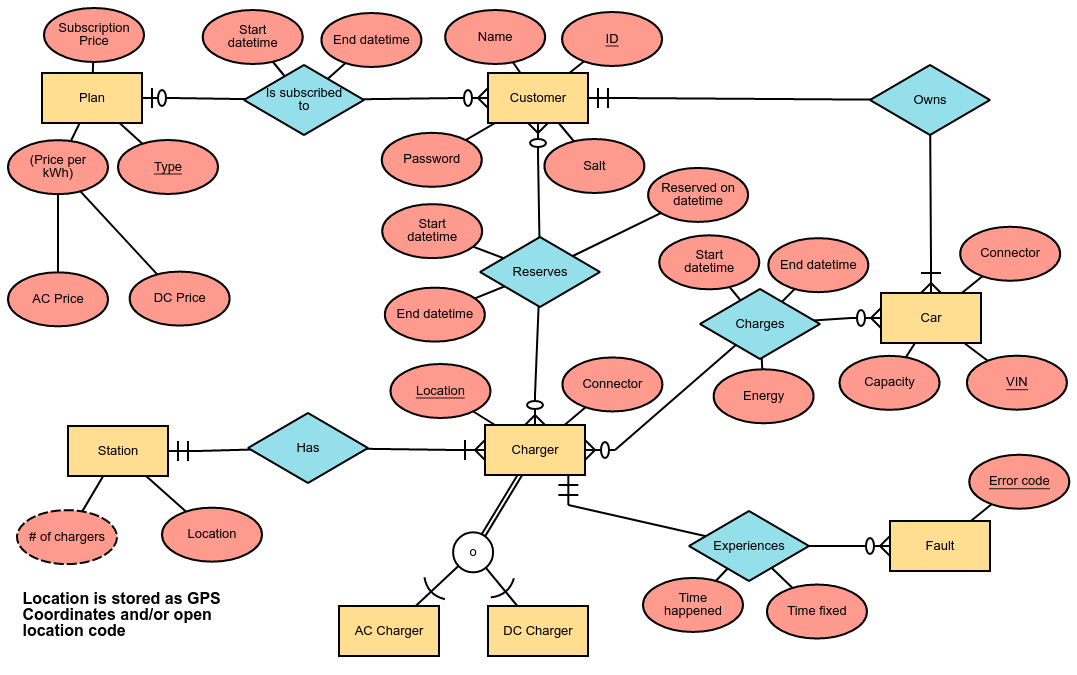
\includegraphics[width=1.1\textwidth]{../img/Charging Stations.png}
    \end{figure}
    \end{adjustwidth*}

\end{frame}

\begin{frame}
    \frametitle{Σχεσιολογικο Μοντελο }

    \begin{adjustwidth*}{-3cm}{-3cm}
    \begin{figure}
        \centering
        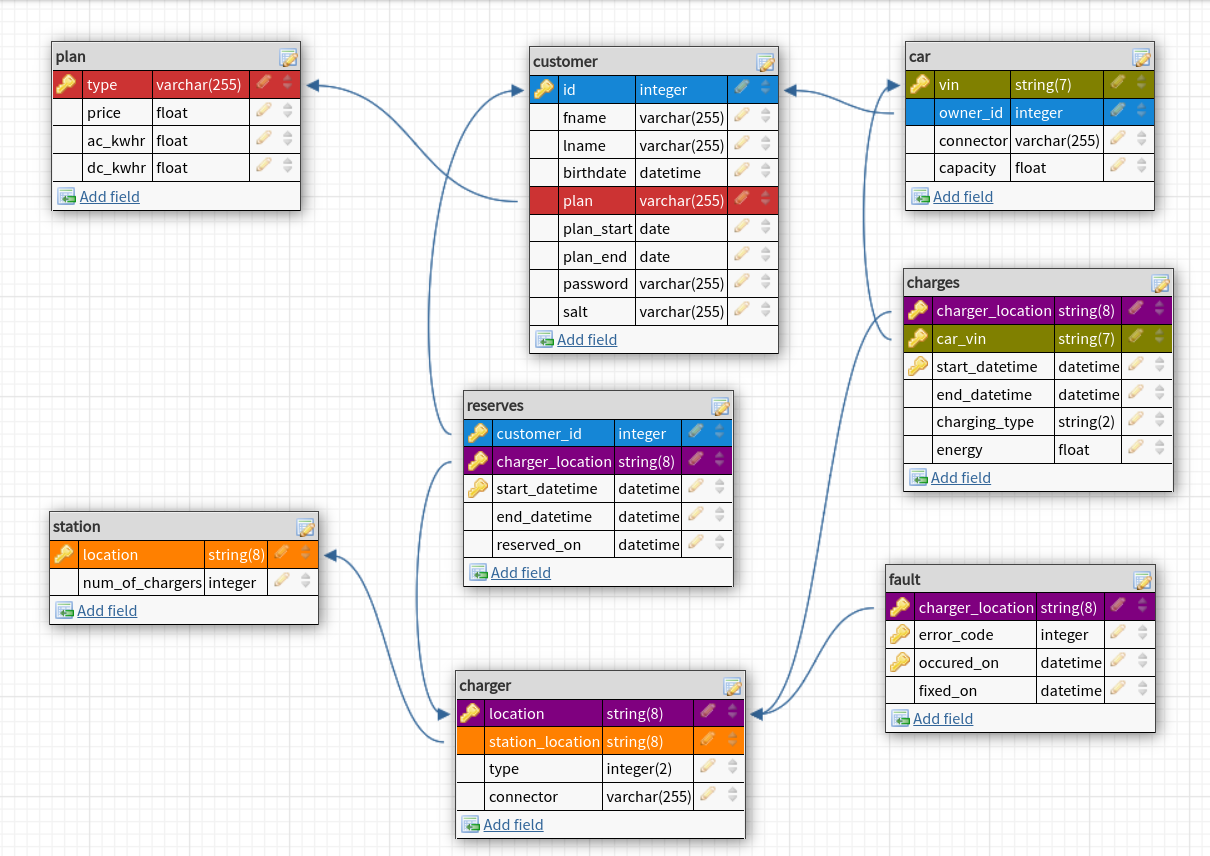
\includegraphics[width=1.1\textwidth]{../img/DBDesigner.png}
    \end{figure}
    \end{adjustwidth*}

\end{frame}


\begin{frame}
    \frametitle{Πληροφορίες που παρέχει η βαση δεδομενων}

    \begin{itemize}
        \item Αριθμός φορτιστών με βάση τον τύπο τους
        \item Πόσα οχήματα φορτίζονται αυτή τη στιγμή
        \item Πόση είναι η συνολική ενέργεια που έχει καταναλωθεί
        \item Ποιος σταθμός καταναλώνει περισσότερη ενέργεια το μήνα
        \item Ώρες αιχμής κάθε σταθμού ή όλου του συστήματος
        \item Μέσος όρος χρόνου ανάμεσα σε σφάλματα
        \item Μέσος όρος kWh ανάμεσα σε σφάλματα
        \item Έσοδα ενός σταθμού

    \end{itemize}
\end{frame}



\begin{frame}
    \frametitle{Πληροφορίες που παρέχει η εφαρμογη}

    \begin{itemize}
        \item Η περισσοτερο και λιγοτερο συχνη ωρα φορτισης
        \item Ποσοι ειναι οι διαθεσιμοι φορτιστες αναλογα με τον τυπο
        \item Πόση είναι η συνολική ενέργεια που έχει καταναλωθεί
        \item Ποιος σταθμος εχει το μεγαλυτερο κερδος
        \item Ποιος ειναι ο μεσος ορος αναμεσα σε σφαλματα φορτιστων
    \end{itemize}
\end{frame}

\begin{frame}
    \frametitle{Δυνατοτητες Εφαρμογης}
    \begin{itemize}
        \item Διαχειριση Των χρηστων και των οχηματων τους με κρυπτογραφηση των κωδικων 
        \item Ο διαχειριστης της βασης μπορει να διορθωσει τα σφαλματα που εχουν προκυψει απο στους διαφορους σταθμους 
        \item Στατιστικα στοιχεια 
        \item Ασφαλεια στην διαχειριση των ερωτηματων προς την βαση δεδομενων 
    \end{itemize}
\end{frame}


\begin{frame}
    \frametitle{Main}

    \begin{adjustwidth*}{-3cm}{-3cm}
    \begin{figure}
        \centering
        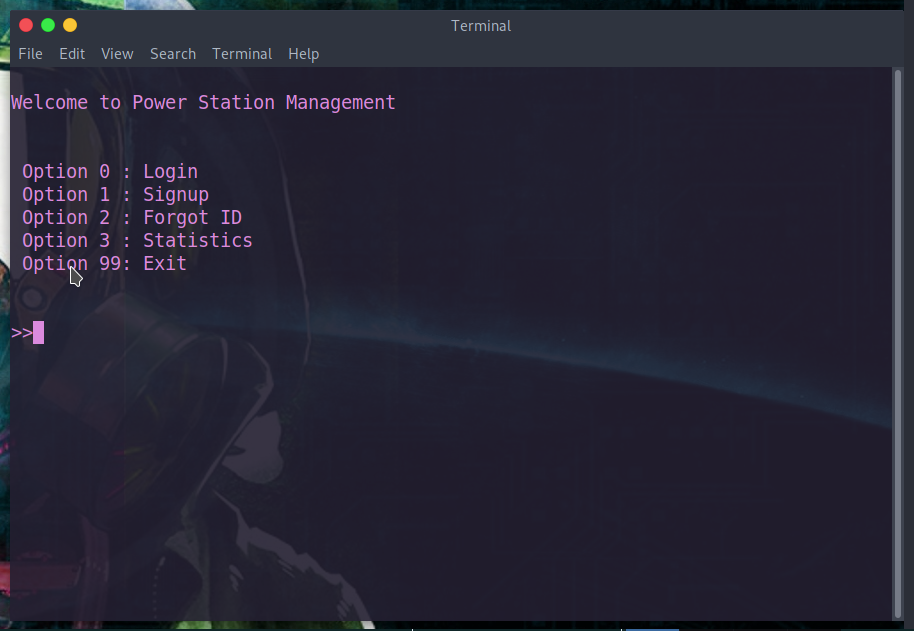
\includegraphics[width=1.1\textwidth]{../img/db_main_page.png}
    \end{figure}
    \end{adjustwidth*}

\end{frame}

\end{document}
